%!TEX root = ../sbc-template.tex

\emph{Machine Learning} (ML), também chamado de Aprendizado de Máquina, é uma subárea da Inteligência Artificial que trata do estudo sistemático de algoritmos e sistemas que são capazes de melhorar seu desempenho com a experiência. Um algoritmo que tem este comportamento é aquele capaz de aprender a partir de dados, assim como humanos e outros animais. Estes, ao se depararem com determinada situação, costumam procurar lembranças de situações similares, de como agiram, e se o comportamento adotado foi vantajoso, e deve ser repetido, ou prejudicial, devendo ser evitado \cite{marsland2015machine}, \cite{goodfellow2016deep}, \cite{flach2012machine}.

De maneira análoga ao aprendizado natural, os algoritmos de \emph{machine learning} precisam aprender, processo chamado de aquisição da experiência. De acordo com a definição clássica de  \cite{mitchell1997machine}, um algoritmo que aprende a partir da experiência $E$ quanto a um conjunto de tarefas $T$ e medida de performance $P$, se sua performance nas tarefas em $T$, medida por $P$, melhora com a experiência $E$.

Ao inferir um algoritmo de \emph{machine learning} para desenvolver determinada tarefa, busca-se um modelo, ou seja, uma função, que mapeie as instâncias do espaço de entrada para o de saída \cite{flach2012machine}. Estes modelos podem ser agrupados em diferentes categorias ao se considerar o tipo de aprendizado e de saída desejada para o algoritmo. Na Figura \ref{fig:ml_algorithms} está uma visão geral dos modelos de algoritmos de \emph{machine learning} e suas subdivisões.

\begin{sidewaysfigure}
	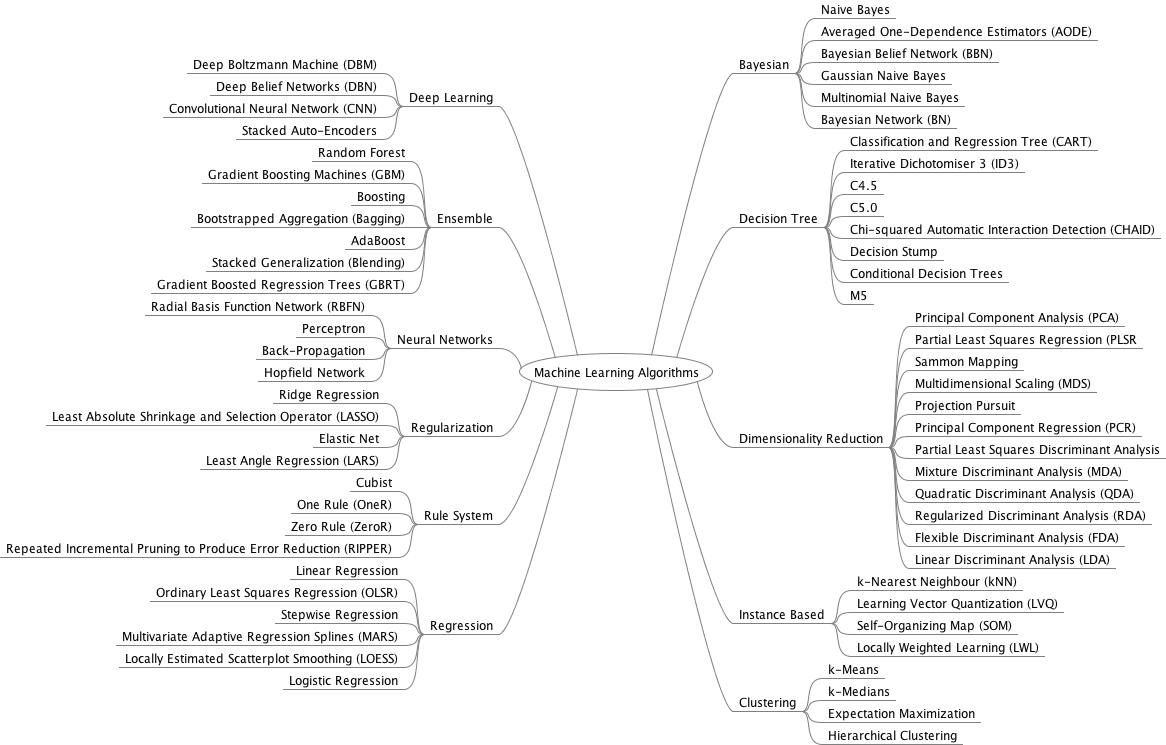
\includegraphics[width=\linewidth]{img/machinelearningalgorithms.png}
	\caption{Mapa mental dos algoritmos de \emph{Machine Learning} organizados por área e sub-área.}
	\label{fig:ml_algorithms}
\end{sidewaysfigure}


Quanto ao tipo de aprendizado, as tarefas de \emph{machine learning} podem ser agrupadas em três tipos diferentes, a depender da presença e do tipo de resposta dada ao algoritmo quanto ao desempenho de suas saídas. No aprendizado supervisionado o algoritmo deve aprender a inferir valores a partir de dados rotulados, ou seja, que têm seus valores de saída conhecidos, apresentados na fase de treinamento, a exemplo das máquinas de vetores de suporte, redes neurais artificiais \emph{feed-forward}, regressão linear e logística, etc. Já no aprendizado não-supervisionado, o algoritmo deve inferir padrões e estruturas a partir de dados não tabelados, a exemplo de modelos como \emph{k-means}, redes neurais artificiais profundas de codificação preditivas e detecção de anomalia. Por fim, no aprendizado por reforço o algoritmo não recebe dados ou rótulos, e deve aprender a partir das recompensas positivas ou negativas dadas por ações que modifiquem o ambiente de maneira satisfatória ou não \cite{flach2012machine}.

Quanto ao tipo de saída desejado, os problemas podem ser atacados são a classificação, regressão, transcrição, tradução automática, detecção de anomalia, síntese e amostragem. As principais tarefas que podem ser endereçadas utilizando aprendizado supervisionado são a classificação e a regressão \cite{flach2012machine}. Um algoritmo proposto a uma tarefa de classificação deve especificar cada entrada $x$ como pertencente a uma dentre $k$ categoritas pré-determinadas, produzindo uma saída $y=f(x)$ tal que a função $f$ é definida como $f: \mathds{R}^n \rightarrow \{1, \ldots, k\}$, ou seja, $f$ mapeia sequências de números reais  $x$ de dimensão $n$ para um valor $y$ do meio de $k$ possibilidades \cite{goodfellow2016deep}. Dentre as tarefas de classificação estão o reconhecimento de objetos em uma imagem, determinar se um indivíduo será ou não vítima de determinada doença, se sobreviverá ou não a determinado acidente, etc. Uma tarefa de regressão envolve aprender uma função de valor real a partir de uma entrada \cite{flach2012machine}. Assim, a saída $y=f(x)$ é dada pela função $f: \mathds{R}^n \rightarrow \mathds{R}$, ou seja, $f$ mapeia uma entrada multidimensional $x$ para um valor $y$ real  \cite{goodfellow2016deep}. Algumas tarefas de regressão envolvem a previsão de preços de um mercado de ações, a determinação do risco do seguro para um carro, do volume diário de precipitação em determinada cidade, etc.

Os modelos de ML podem ser paramétricos ou não paramétricos. Segundo \cite{russell2016artificial}, um modelo de aprendizado que resume dados utilizando um conjunto de parâmetros de tamanho definidos independente do número de exemplis de treinamento é chamado de \emph{modelo paramétrico}. Dentre os modelos paramétricos estão a regressão linear e as redes neurais artificiais. Já um \emph{modelo não-paramétrico} é aquele que não pode ser caracterizado por um conjunto limitado de parâmetros. Alguns exemplos de modelos não-paramétricos são máquinas de vetores de suporte, k-NN e árvores de decisão CART e C4.5.


Dentre os modelos paramétricos, as redes neurais artificiais (RNAs) têm demonstrado resultados satisfatórios em tarefas de classificação e regressão, em aplicações em diversas áreas. Em especial, aplicações de \emph{Deep Learning} (DL) no reconhecimento de objetos, no processamento de linguagens naturais e \emph{speech recognition} têm trazido ainda mais atenção ao modelo. 
